
\documentclass[a4paper,12pt, twoside]{article}
\usepackage{polski}
\usepackage[utf8]{inputenc}
\usepackage{listings}
\usepackage{graphicx}

\usepackage{xcolor} % Required for specifying custom colors
\usepackage{fix-cm} % Allows increasing the font size of specific fonts beyond LaTeX default specifications

%\setlength\parindent{125cp}
\graphicspath{ {zdj/} }
\renewcommand*{\figurename}{Ilustracja} %zmiana rysunek na ilustrracja przy opsie
\usepackage{subcaption}
\usepackage[export]{adjustbox}
\usepackage{geometry}
\usepackage{titlesec}
\usepackage{fancyhdr}
\pagestyle{fancy}
\renewcommand{\sectionmark}[1]{\markright{#1}}		%aby nie było0.1.2
\fancyfoot[LE,RO]{\thepage}		%numeracja lewo prawo(strona)
\let\oldsection\section		%nowa strona dla sekcji
\renewcommand\section{\clearpage\oldsection}%nowa strona dla sekcji
\renewcommand{\subsectionmark}[1]{}%nazwa rozdziału w nagólwku
\usepackage[section]{placeins}
%\renewcommand{\section}
\titlelabel{\thetitle.\quad}%dodawankie kropki
\rhead{\fancyplain{}{}} % predefined ()
\fancyhead[CE]{Elektronika}
\fancyhead[CO]{\rightmark }
%\chead{\fancyplain{}{\rightmark }} % 1. sectionname
\cfoot{\fancyplain{}{}} %środek stopki
\lhead{\fancyplain{}{}} %lewa część nagłówka
\usepackage[nottoc]{tocbibind}  %opening
\setlength{\parindent}{2em}
\usepackage{indentfirst}
\setlength{\oddsidemargin}{0mm} % Adjust margins to center the colored title box
\setlength{\evensidemargin}{0mm} % Margins on even pages - only necessary if adding more content to this template

\newcommand{\HRule}[1]{\hfill \rule{0.2\linewidth}{#1}} % Horizontal rule at the bottom of the page, adjust width here

\definecolor{grey}{rgb}{0.9,0.9,0.9} % Color of the box surrounding the title - these values can be changed to give the box a different color

\begin{document}

 % Remove page numbering on this page

%----------------------------------------------------------------------------------------
% TITLE SECTION
%----------------------------------------------------------------------------------------
\begin{titlepage}
\small Gimnazjum nr 3 w Zabrzu\\
\line(1,0){431}\\
\colorbox{grey}{
	\parbox[t]{1.0\linewidth}{
		\centering \fontsize{50pt}{80pt}\selectfont % The first argument for fontsize is the font size of the text and the second is the line spacing - you may need to play with these for your particular title
		\vspace*{0.7cm} % Space between the start of the title and the top of the grey box
		
		\hfill Projekt \\
		\hfill Elektronika \\

		\vspace*{0.7cm} % Space between the end of the title and the bottom of the grey box
	}
}

%----------------------------------------------------------------------------------------
\vfill % Space between the title box and author information

%----------------------------------------------------------------------------------------
%	AUTHOR NAME AND INFORMATION SECTION
%----------------------------------------------------------------------------------------

{\centering \large 
\hfill Autorzy: \\
\hfill Bartek Mazur \\
\hfill Krzyś Dziembała \\
\hfill \\
\hfill Klasa 3gb\\

\HRule{1pt}} % Horizontal line, thickness changed here

%----------------------------------------------------------------------------------------

\begin{tabular}{r}
\small\today
\end{tabular}
\hfill
\clearpage % Whitespace to the end of the page

\end{titlepage}
\newpage\null\thispagestyle{empty}\newpage
%\begin{abstract}

%\end{abstract}

\tableofcontents 
\addcontentsline{toc}{section}{Wstęp}
%\addtocontents{toc}{\protect\thispagestyle{empty}}
\thispagestyle {empty}

\section*{Wstęp}
Ten projekt jest dedykowany ludziom na każdym poziomie znajomości tematu. Przez kolejne rozdziały będziemy uzupełniać podstawowe informacje potrzebne do zbudowania prostych układów elektronicznych, aby w kolejnej części zacząć przedstawiać podstawowe schematy i proste programy. Doświadczony w tej dziedzinie czytelnik może je po prostu pominąć (nie wszyscy chcą się uczyć programowania schematami blokowymi). 
*Nota dla zaawansowanych czytelników:
Używamy procesorów "atmel", a do programowania środowiska Arduino. Cały kod używany w prezentacji będzie udostępniony na GitHub'ie.

\section{Programowanie Arduino}

Arduino aby działać musi zostać zaprogramowane. Programuje się je w języku Arduino, opartym na językach C/C++.
Program jest kompilowany, czyli przetwarzany na język zrozumiały dla urządzenia, oraz na nie wgrywany za pomocą
Arduino IDE, o którym więcej w sekcji "Środowisko". 

%![Arduino IDE](https://www.arduino.cc/en/pub/skins/arduinoWide/img/ArduinoAPP-01.svg)
Kolejny akapit

\subsection {Składnia języka używanego w środowisku C++}
%Największą różnicą jest struktura, składnia praktycznie się nie różni - CO TU CHCIAŁEŚ NAPISAĆ???
  Język Arduino można podzielić na 3 główne części:
  \begin{enumerate}
	\item Struktura
	\item Zmienne
	\item Funkcje
\end{enumerate}
\subsubsection  {Struktura}
																											%\begin{figure}
																												%\centering
																													%\includegraphics{../../Users/Madar/Desktop/bartek_pulpit/zdjęcia/bartek.jpg}
																												%\label{fig:bartek}
																											%\end{figure}
	Aby program działał niezbędne są dwie funkcje:
	\renewcommand{\labelitemii}{$\circ$}
	\begin{itemize}
	
	  \item void setup() - wykonywana tylko raz na początku programu
		
	  \item void loop() - wykonywana cały czas po wykonaniu funkcji "setup"
	 
	\end{itemize}
	  %przykładowy kod
	Wśród struktur możemy wyróżnić także:

	\begin{itemize}
		\item if(){} - wykonuje kod zawarty w nawiasach klamrowych, jeśli warunek w zwykłych nawiasach jest spełniony. Do porównania wartości stosuje się:
			\begin{itemize}
				\item \verb|>| - jest większe
				\item \verb|<|  - jest mniejsze
				\item == - jest równe
				\item != - jest różne od
				\item \verb|<=| - mniejsze bądź równe
				\item \verb|>=| - większe bądź równe
			\end{itemize}
		\item else - wykonuje kod zawarty w nawiasach klamrowych, jeśli warunek w if nie jest spełniony. \textbf{Używany tylko razem z "if".} Przykład:
		\begin{verbatim}
		if(x > y){
		  Serial.println("x jest większe od y.");
		} else {
		  Serial.println("x nie jest większe od y.");
		}
		\end{verbatim}
		\item for - jest to pętla, której zawartość w klamrach zostanie tyle razy wykonana, ile razy spełniony jest warunek podany na wejściu. Budowa:\\*
		for(indeks, warunek dla którego funkcja ma się wykonywać, co zrobić z indeksem po wykonaniu){}\\*
		Przykład pętli for, która wypisze wartości od 0 do 2 włącznie:
		\begin{verbatim}
		for (int x=0;x<3;x++){
		  Serial.println(x);
		}
		\end{verbatim}
		\item while() - pętla, która wykonuje kod w nawiasach klamrowych, jeśli warunek w zwykłych nawiasach jest spełniony.\\*
		Przykład pętli while wypisującej wartości zmiennej x i zwiększającej tę wartość jeśli jest ona mniejsza niż 3:
		\begin{verbatim}while(x<3){
		  Serial.println(x);
		  x++;
		}
		\end{verbatim}
		\item do... while() - pętla podobna do pętli "while", ale kod zostanie wykonany co najmniej raz, nawet jeśli warunek nie jest spełniony. \\*
		Przykład pętli do... while, która wypisze wartość x tylko raz (choć warunek \textbf{nie} jest spełniony):
		\begin {verbatim}
		int x = 3;
		do{
		  Serial.println(x);
		}while(x<1);
		\end{verbatim}
		
	\end{itemize}
	Do tej kategorii możemy zaliczyć także niektóre symbole:
	\begin{itemize}
		\item ; - stawiany na końcu każdej (nie pustej) linii kodu. Nie jest niezbędny, jeśli linia jest zakończona znakiem \}
		\item \{\} - w nawiasach klamrowych jest zawarty kod każdej funkcji, pętli i "if", oraz "else"
		\item // - stawia się przed komentarzem. Ten typ komentarzy zaczyna się od tych znaków i kończy się z końcem linijki. \textbf{Komentarze są ignorowane przez kompilator} 
		\item /**/ - komentarz wieloliniowy. Komentarz wstawia się za "/*", a kończy się go "*/".
		\item = - przypisuje zmiennej określoną wartość. Przykład przypisania zmiennej "x" typu "string" wartości "wartość":
			\begin{verbatim}
			string x = "wartość";
			\end{verbatim}
		\item + - oznacza dodawanie
		\item - - oznacza operację odejmowania
		\item * - mnożenie
		\item / - dzielenie
		\item \% - modulo (reszta z dzielenia). Działanie: x \% y - reszta z dzielenia x przez y
		\item ++ - powiększ o 1. Przykład kodu zwiększającego zmienną x o 1:
			\begin{verbatim}
			x++;
			\end{verbatim}
		\item -- - zmniejsz o 1. Wykorzystanie w ten sam sposób co --
		\item += - powiększ o. Przykład kodu zwiększającego zmienną x o 7:
			\begin{verbatim}
			x+=7;
			\end{verbatim}
			Równoważne z kodem
			\begin{verbatim}
			x = x + 7;
			\end{verbatim}
		\item -= - pomniejsz o. "x -= y" jest równoważne z "x = x - y"
		\item *= - przemnóż przez. "x *= y" równoważne do "x = x*y"
		\item /= - podziel przez. "x /= y" = "x = x/y"
		\item \%= - zapisz jako resztę z dzielenia przez. "x \%= y" jest równoważne z "x = x\%y".
	\end{itemize}
	Należy pamiętać również o:
	\begin{itemize}
		\item \#include - używany na początku kodu przed jakąkolwiek funkcją, aby dołączyć biblioteki. \textbf{Nie stawiamy po nim średnika!} Przykład:
			\begin{verbatim}
				\#include <Keyboard.h> //dodaje bibliotekę wprowadzającą obsługę klawiatury
			\end{verbatim}
		\item \#define - używany na samym początku kodu prze jakąkolwiek funkcją. Za jego pomocą możemy zdefiniować jaką wartość będzie mieć fragment tekstu.
		Działa tak jakby zamiast ciągu znaków zaraz po słowie "define" były te oddzielone od nich spacją. \textbf{Nie stawiamy po nim średnika!} Przykład kodu wypisującego co 1s tekst zdefiniowany na początku.
			\begin{verbatim}
				#define tekst "Hej!"
				#define przerwa 1000
				
				void setup(){
				  Serial.begin(9600);
				}
				void loop(){
				  Serial.println(tekst);
				  delay(przerwa);
				}
			\end{verbatim}
	\end{itemize}
	\subsubsection{Zmienne}
		Dane przetwarzane przez program przechowywane są jako zmienne. W zależności od rodzaju zmiennej może ona przechowywać różne wartości.
		\\*Wyróżniamy następujące typy zmiennych:
		\begin{itemize}
			\item void - używany tylko do tworzenia funkcji, które nie zwracają żadnej wartości.
			\item boolean - zmienne typu boolean przechowują tylko wartości \textbf{true} i \textbf{false}. Zamiast "false" można użyć 0, a każda niezerowa liczba zostanie uznana za "true".
			\item char - typ danych zawierający bajt pamięci. Przechowuje wartość znaku.
				Podczas nadawania zmiennej wartości należy zapisać ją w pojedynczym cudzysłowie.
				Jednak znaki przechowywane są jako odpowiadające im liczby zgodnie z kodowaniem ASCII.
				Zmienna "char znak = 'A';" może być zapisana również tak: "char znak = 65;".
				Korzystając z tej własności możemy np pisząc "znak += 32;" zmienić wartość tej zmiennej z 'A' na 'a', czyli zmienić dużą literą na małą (i odwrotnie).
			\item byte oraz unsigned char - przechowuje 8 bitową liczbą od 0 do 255. Zalecane jest używanie "byte" zamiast "unsigned char".
			\item int - przechowuje wartości liczbowe. Zakres wartości zależy od procesora.
				Dla Arduino Uno (i innych urządzeniach opartych na procesorze ATMega) jest 16-bitowa i ma zakres od -32768 do 32767.
			\item word oraz unsigned int - od zwykłego różni się tym, że przechowuje tylko wartości nieujemne.
				Jego zakres dla Arduino Uno i innych Arduino opartych na procesorach ATMega jest od 0 do 65535.
			\item long - przechowuje wartości liczbowe. Ma rozmiar 32 bitów. Przyjmuje wartości od -2147483648 to 2147483647. Po liczbie należy dać literę "L" (long liczba = 51523487L).
			\item unsigned long przechowuje 32 bitową liczbę. Ma zakres od 0 do 4294967295.
			\item short - dla wszystkich Arduino jest taki sam jak int na procesorach ATMega.
			\item float - typ zmiennej dla liczb zmiennoprzecinkowych. Zajmują 32 bity pamięci. Mogą przechowywać wartości od -34028235E+38 do 3.4028235E+38. Liczby zmiennoprzecinkowe \textbf{nie są dokładne}!
				Na przykład "6.0 / 3.0" może nie być równe "2.0". Mają dokładność \textbf{tylko 6-7 cyfr znaczących}! Operacje na zmiennych zmiennoprzecinkowych \textbf{trwają dłużej} niż na liczbach całkowitych.
				Należy również pamiętać, że nie umieszczenie kropki przy podawaniu wartości spowoduje, że zmienna traktowana będzie jako "int".
			\item double - zmienna zmiennoprzecinkowa o podwójnej dokładności względem "float". Na procesorach ATMega zajmuje 32 bity pamięci, a na Arduino Due 64 bity.
				\textbf{W przypadku Arduino NIE jest dokładniejsza od zmiennej typu "float".}
			\item string - tablica znaków. Najprościej tworzy się ją tak:
				\begin{verbatim}
				char nazwa[] = "Zawartość zmiennej nazwa";
				\end{verbatim}
			%##############################################################
			%Dokończ string (tablicę), zrób string (obiekt) i napisz dalej
			%##############################################################

		\end{itemize}


%to do bibliografi[https://www.arduino.cc/en/Guide/Introduction, https://www.arduino.cc/en/Reference/HomePage]

	\subsection {Styl pisania}
	Nie mówimy tutaj czysto o algorytmice (przeszukiwanie danych, analiza obrazu itp.) jednak jest pewien schemat postępowania. Arduino składa się z czujników (sensorów) oraz odbiorników. %spis tego na samym końcu
	\\
	Możemy  na bieżąco analizować i przetwarzać dane. Na samym początku może się to wydawać niezrozumiałe ale przy odrobinie wprawy i obycia z urządzeniem zmienią podejście.
		
	Podstawą jest umiejętność skonstruowania algorytmu, czyli ciągu poleceń do wykonania. Można zapisać to tak:
	\\Czytaj wartość czujnika \verb|->| analiza \verb|->| akcja zależna od wyniku analizy (np. zapal światło, włącz silnik).
%W ogólniej wersji wygląda to tak:
\subsubsection{Schemat ogólny}
	Przyjrzymy się ogólnej postaci programów. Zostaną one wytłumaczone na przykładzie schematu blokowego aby nawet niewprawiony czytelnik był w stanie cokolwiek zrozumieć.
\subsubsection{Przykłady z życia wzięte}
W tej części przeanalizujemy kod "normalnie" używany
%CZytaj wartość czujnika -> analiza -> sygnał do odbiornika(zgaś światło, rusz silnikiem)
	%\subsection{Jezyk używany}
	\subsection{Środowisko}
	Środowisko - miejsce w którym dzieją się cuda, a mianowicie powstają nasze programy. Jak każdy język, Arduino również ma własne środowisko (Arduino IDE).
	Środowisko umożliwia nam edytowanie programów oraz kompilację i wgrywanie ich na urządzenie %(odnośniki do wyższego rozdziału tutaj powinny się znajdować)
		Wygląda ono w ten sposób: screen z Arduino. 
	\subsubsection{Skąd pobrać}
	Pobieramy je ze strony (odnośnik w przypisach) zgodne z wersją naszego systemu operacyjnego. Następnie instalujemy, wykonując polecenia instalatora
	ew. (w przypadku Windowsa) rozpakowujemy zip'a do dowolnej lokalizacji i z niej uruchamiamy arduino.exe.
\subsubsection{Pierwsze kroki}
Programowanie jest intuicyjne ale musimy pamiętać o kilku rzeczach. A mianowicie należy ustawić płytkę (zdj. numer),  port szeregowy (zdj. numer)% i coś jeszcze
%(zdjęcia z tego razem z podpisem)


%---Do bibliografii-----------------------------------
\cite{Introduction, Reference}
%-----------------------------------------------------


\begin{figure} %     
%  \centering
  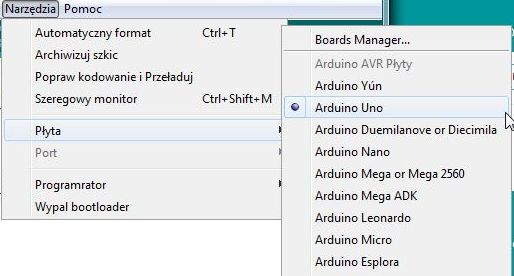
\includegraphics[scale=0.7]{arduino-ustawPlytke.jpg}
  \caption{Ustawianie płytki}
  \label{fig:test}
	\end{figure}
	\begin{figure}
%  \centering
  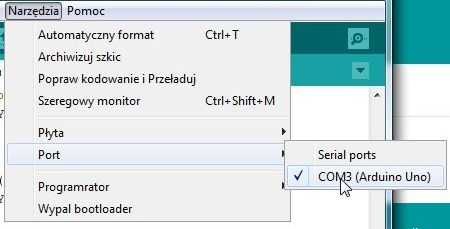
\includegraphics[scale=0.7]{arduino-ustawPort.jpg}
  \caption{Ustawianie portu}
  \label{fig:test}
\end{figure}


\section{Podstawy elektroniki}
 \subsection{Fizyka w elektronice}
	Fizyka w elektronice nie różni się od tej poznanej w gimnazjum. Był cały dział 'prąd'. Ten dział właśnie nam się przyda. Nie zagłębiając się we wszystkie szczegóły, powtórzymy prawo Ohma:
	\begin{center}
	\[
	I=\frac{U}{R}
	\]	
	\end{center}
Zadanie z tym związane (pojęcia będą wytłumaczone w dalszej części): \\* Mamy diodę oraz źródło zasilania 5V. Jaki rezystor musimy podłączyć aby prąd płynący przez diodę był ok 20mA %do sprawdzenia
%pracowało na prąd stały lub zmienny (podłączamy do gniazdka lub zasilanie z baterii - prosto tłumacząc).
	\subsection{Elementy elektroniczne i ich symbole}
	\subsubsection {Symbole}
	Elektronika ma swój własny język.Przypomnijmy oznaczenia niektórych elementów z elektroniki:
\begin{itemize}
	\item sym.-dioda świecąca
	\item sym.-źródło prądu stałego
	\item sym.-żarówka
	\item sym.-rezystor
\end{itemize}
   \subsubsection{Definicje tych elementów}
	
Żarówka - jest to źródło światła(i ciepła) elektrycznego, poprzez żarzenie się trudno topliwego materiału(często wykorzystywany jest drucik wolframowy przez który płynie duży prąd). Sprawność ok.
8-10 lumenów/wat. 

Źródło prądu stałego - jak nazwa wskazuje jest to miejsce, w którym "powstaje prąd" jednostką jest napięcie wolt[V]. W elektronice powszechnie stosuje się napięcie 3,3V i 5V. Dla porównania w gniazdku jest 220-230V.

Rezystor - jest wykorzystywany do ograniczenia płynącego prądu w obwodzie. Zamienia energię elektryczną w ciepło. (Kolejny rozdział)[jak czytać opór na rezystorze - te paski]

Dioda świecąca - element elektryczny który przewodzi prąd tylko w jedną stronę. Stosowane w wyświetlaczach LED jak również w pilotach (na światło podczerwone) Charakteryzuje się dosyć dużą sprawnością 26-300 lumenów/W. 
%oświetlnie na boiskach sportowych

\subsubsection{Zastosowanie symboli}
    
Do rysowania schematów używamy tych właśnie symboli. Symbole te są znane na całym świecie więc gdy narysujemy (dioda) każdy będzie wiedział, że to dioda. Na początku nie będziemy rysować bardzo skomplikowanych układów ale należy wiedzieć że one istnieją. Przydają się przy czytaniu niektórych instrukcji (np. do jakiegoś czujnika).
%Schem nasz(jeden układ sygnalizatora) i dla porównania schemat (arduino mini- lub czegoś innego)

	\subsection{Jak czytać opór}
Nie ma tutaj żadnej filozofii. Musimy po prostu 'podstawić' nasz opornik i przeczytać. Spróbujcie sami ilustracja x. Rozwiązanie na końcu.

W systemie znakowania paskowym 2 pierwsze paski oznaczają wartość rezystancji którą czytamy jako jedną liczbę, a 3 pasek mnożnik przez który należy pomnożyć te dwie pierwsze liczby.
Czwarty pasek to dopuszczalna tolerancja. - tolerancja to zakres błędu. Np dla opornika 10[ohm] +- 10\% znaczy, że opór będzie nam się wahał od 9-11[ohm].
\begin{figure}
 \centering
  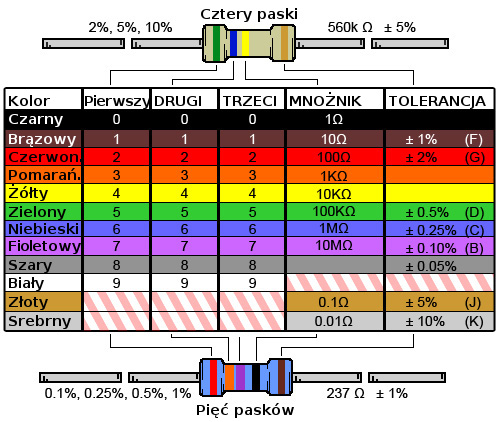
\includegraphics[scale=0.7]{kod_paskowy.jpg}
  \caption{Kod paskowy rezystorów}
  \label{fig:test}
\end{figure}
\begin{figure}
 \centering
  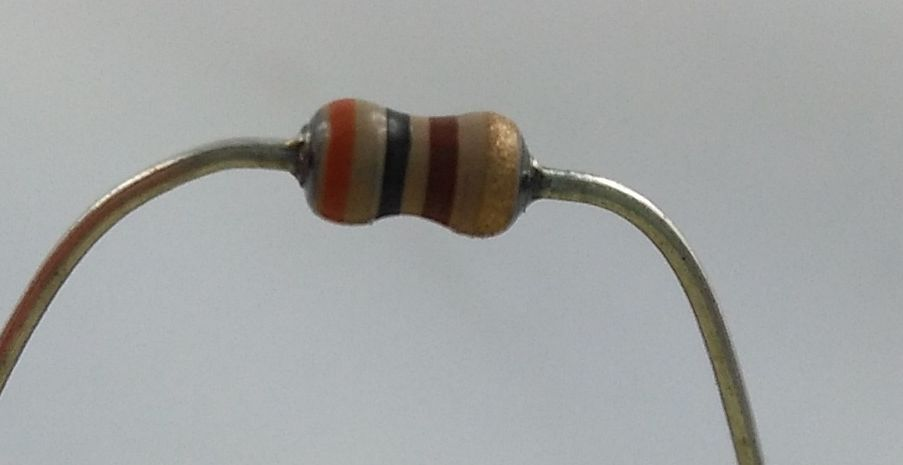
\includegraphics[scale=0.4]{opornik.jpg}
  \caption{Przykładowy rezystor}
  \label{fig:test}
\end{figure}
\FloatBarrier
	\subsection {Domowy warsztat}
    
       \subsubsection{ O co chodzi}
W tym rozdziale czytelnik dowie się jak zacząć przygodę z programowaniem jeśli nigdy nie miał styczności z tym. Po wybraniu swojego poziomu są umieszczone tabelki z zadaniami oraz z listą zakupów .
\subsubsection{Podstawy podstaw - poziom 1}
Jest to idealne połączenie dla czytelników, którzy zaczynają przygodę z elektroniką oraz z programowaniem jednocześnie. Dzięki temu nauczy się podstaw z tych dziedzin. 
To, co czytelnik ma zrobić aby posiąść tę wiedzę będzie omówione w dalszej części dokumentu. Koszyk odpowiedni w na tym poziomie znajdziemy w tab: Zawartość koszyka na poszczególnych poziomach.
Poziom 1:
-któreś Arduino
-płytka stykowa
-kabelki (damsko-męskie i męsko-męskie)
czujnik, oporniki (do diod)
\subsubsection{Advanced beginner - poziom 2}
Czytelnik:
-zna podstawową składnię używaną w Arduino,
-zna różnice między Arduino Nano oraz Arduino Uno,
-potrafi uruchomić diodę wciskając przycisk,
-spędził co najmniej 5h w środowisku Arduino

Gdy czytelnik posiądzie wiedzę minimalną, może przejść do kolejnego poziomu wtajemniczenia w elektronikę, prócz poszerzenia naszego warsztatu, zmiany trudności zadań, czytelnik musi wykazać się swoją kreatywnością, ponieważ w tym momencie pojawiają się schody.

\subsubsection{Expert - poziom 3}
Jako, że jest to poradnik dla początkujących i średnio zaawansowanych, wyróżnimy tylko 3 poziomy wtajemniczenia. W tym poziomie nie ma już stricte list zakupów, ponieważ Expert sam dobrze wie co chce robić. 
\subsubsection{Lista zakupów}
Jak już wcześniej zostało napisane, w tym rozdziale zostanie poruszony temat listy zakupów oraz jak kupować

 Najlepszą stroną do kupowania elektroniki jest allegro, wszystkie dostępne (mniej lub bardziej podstawowe) czujniki znajdziemy w kategorii 'Arduino' (opcjonalnie nazwa czujnika np. magnetometr).

Jeżeli mamy czas i potrzebujemy więcej czujników, najlepiej zamówić je w Chinach poprzez Aliexpress. Nie należy się obawiać, że nie przyjdą jednak musimy uzbroić się w cierpliwość (najdłużej czekałem ok 70 dni).

%tabelka
\subsubsection{Zadania}
Tak jak w przypadku zakupów, problemy zadaniowe mają swoje własne serwisy, które ułatwiają pracę. Jest kilka ważnych zasad związanych z tym: szukamy po angielsku, problem wpisujemy w google i szukamy na Stackoverflow, do Arduino polecam forum Arduino też (przykładowe problemy)
\subsubsection{Reszta śmieci do zedytowania}
Zadania mają charakter edukacyjny i wszystkie uczą różnych knifów w programowaniu Arduino. Czasami jednak czytelnik będzie musiał wykazać się umiejętnością szperania w sieci. Podpowiedzi do zadań będą umieszczone w internecie.
%github, pozdrawaim
Jak zacząć:
Gdy kupiliśmy Arduino Nano wpinamy je jak na zdjęciu (zdj płytka stykowa-Arduino Nano) teraz możemy bez problemu wpiąć inne elementy (zdj serwa i np naszego sygnalizatora)
Gdy kupimy Arduino uno nie potrzebujemy nawet płytki stykowej ponieważ jest ono tak skonstruowane że możemy od razu wpinać urządzenie w płytkę
(znowu zdjęcia ale z uno)
To jest tak jakby wersja testowa. Na płytce stykowej łączymy wszytko kabelkami.
Załącznik lista zakupów: lv1, lv2, lv3


        

\section{Pierwszy mikrokontroler}
		Jest to dość podstawowy element: co trzeba mieć aby zacząć przygodę z elektroniką. Odpowiedz: praktycznie nic. W kolejnych częściach spróbujemy ustalić poziom zaawansowania w czytelnika w elektronice oraz w programowaniu.
\begin{figure}[htb]
  \centering
  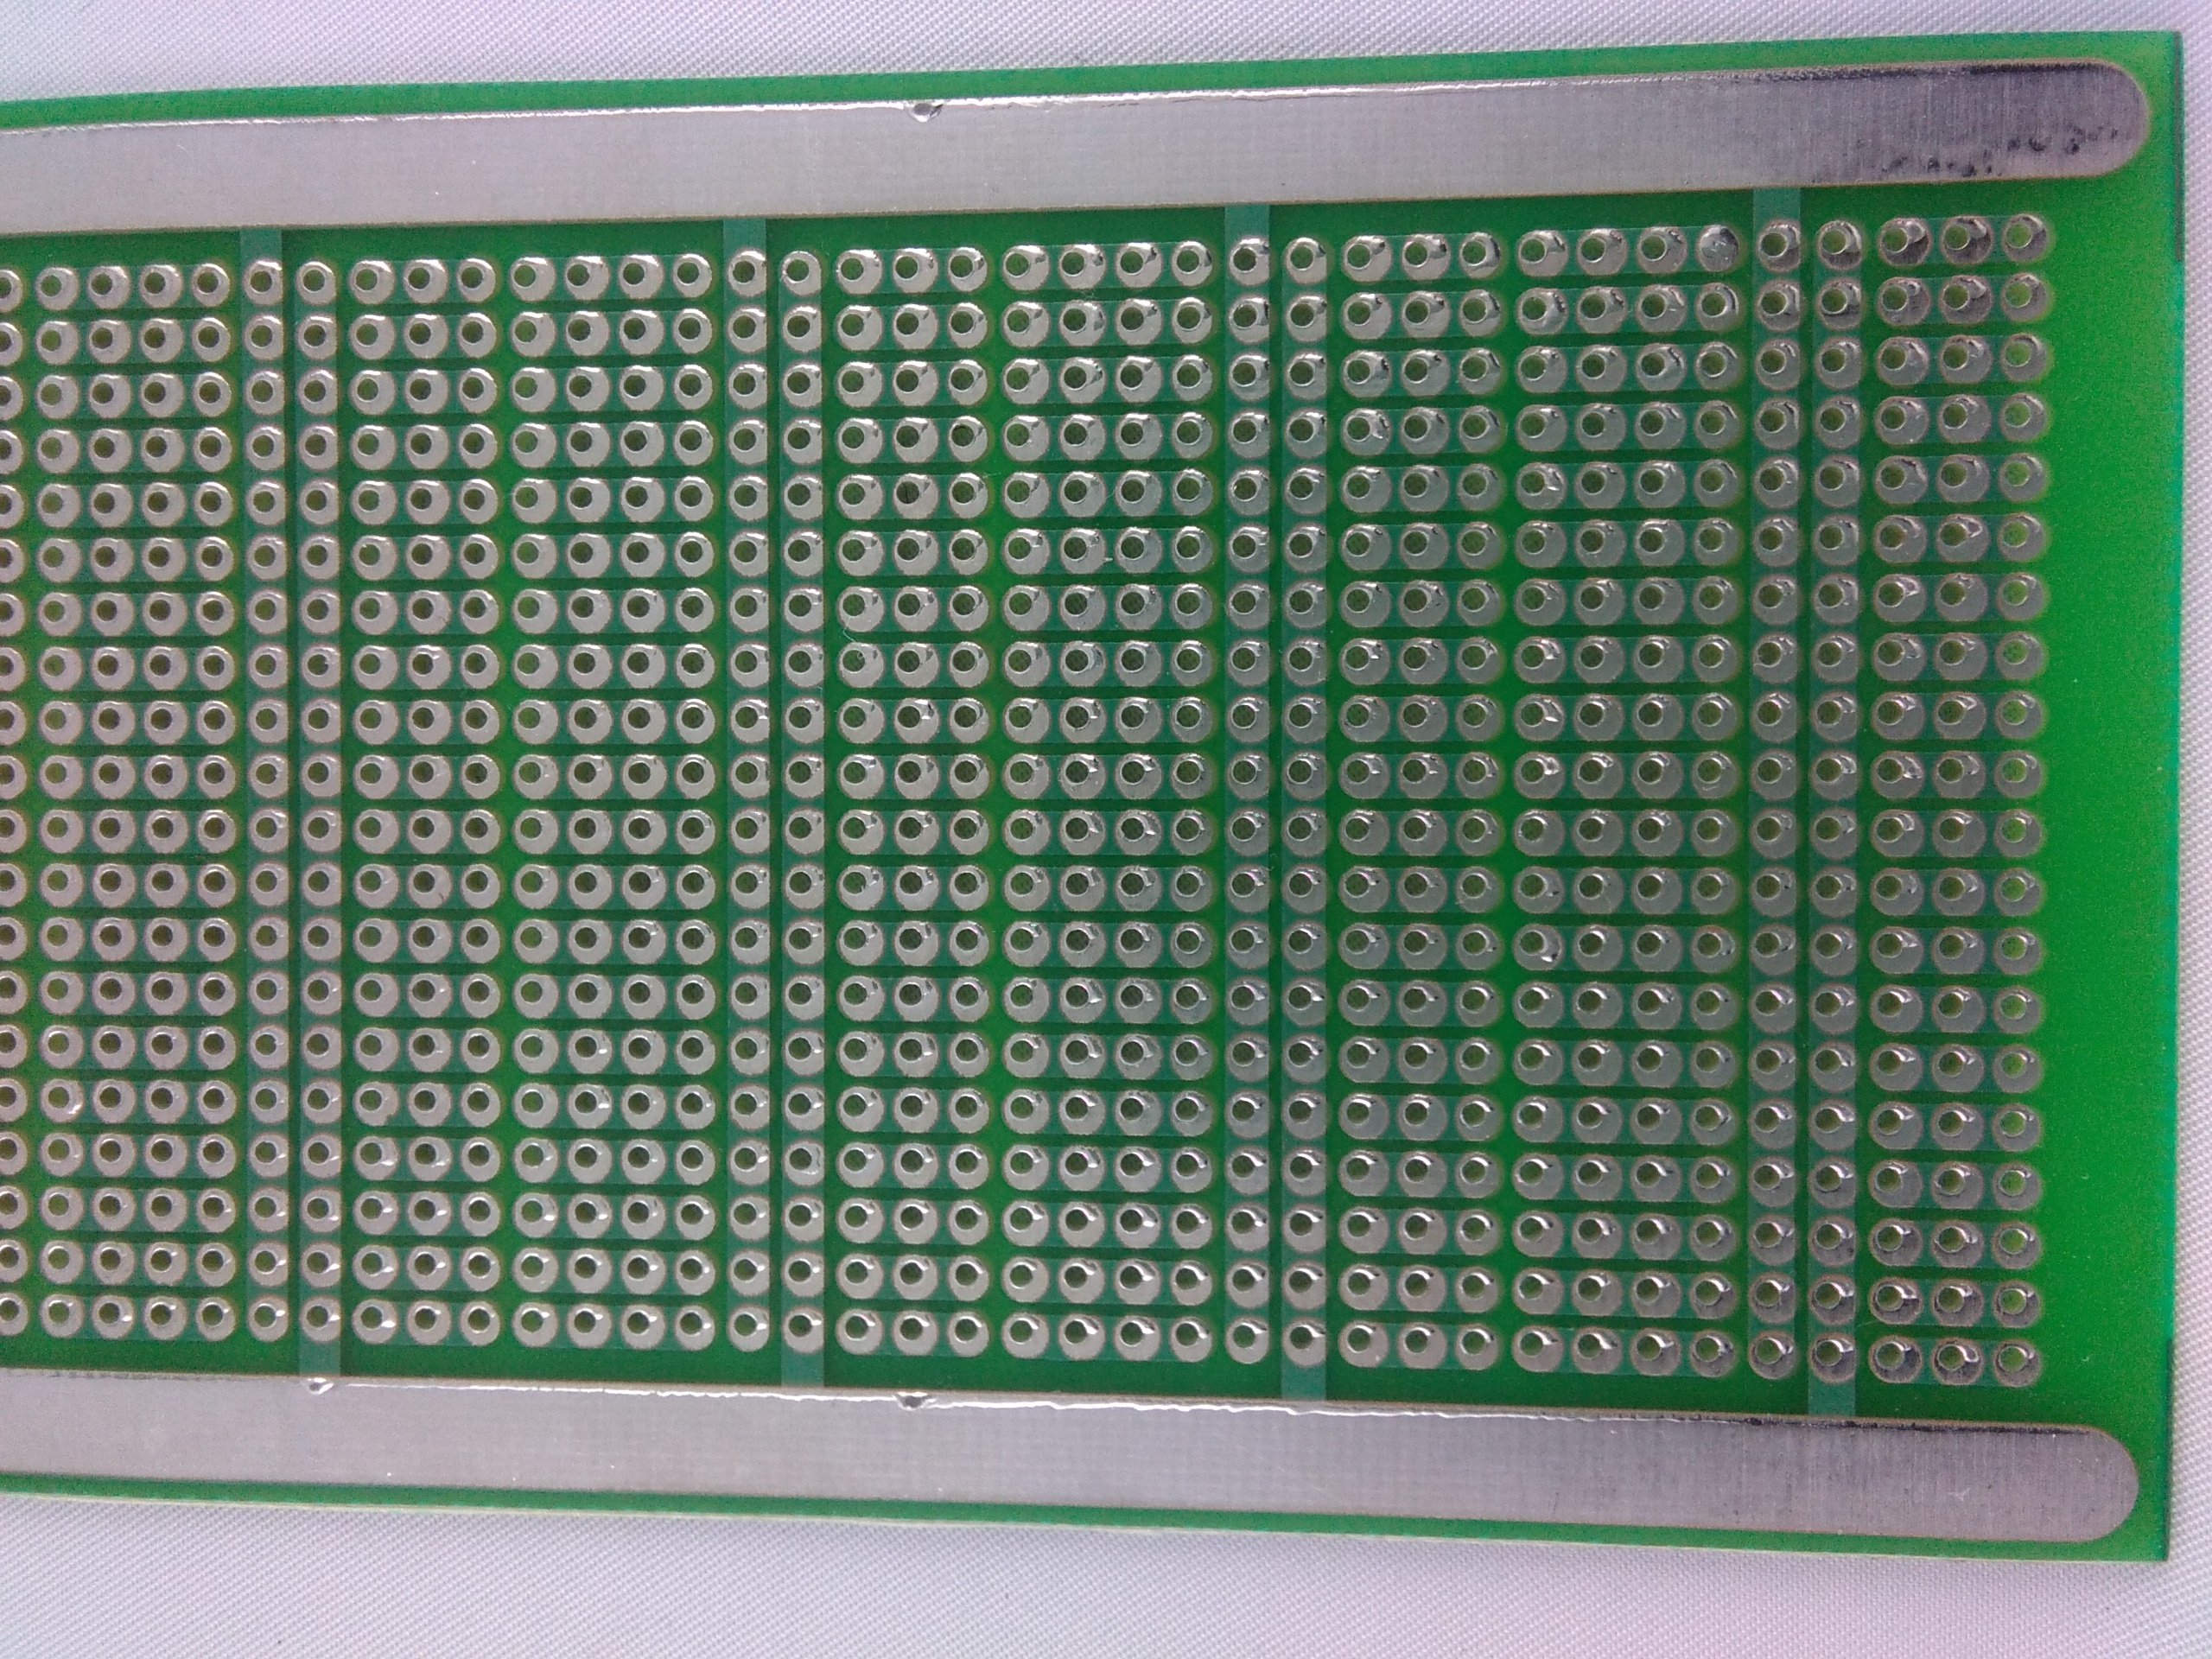
\includegraphics[scale=0.1,right]{universe.jpg}
  \caption{test figure}
  \label{fig:test}
\end{figure}
\begin{figure}[!h]
  \centering
  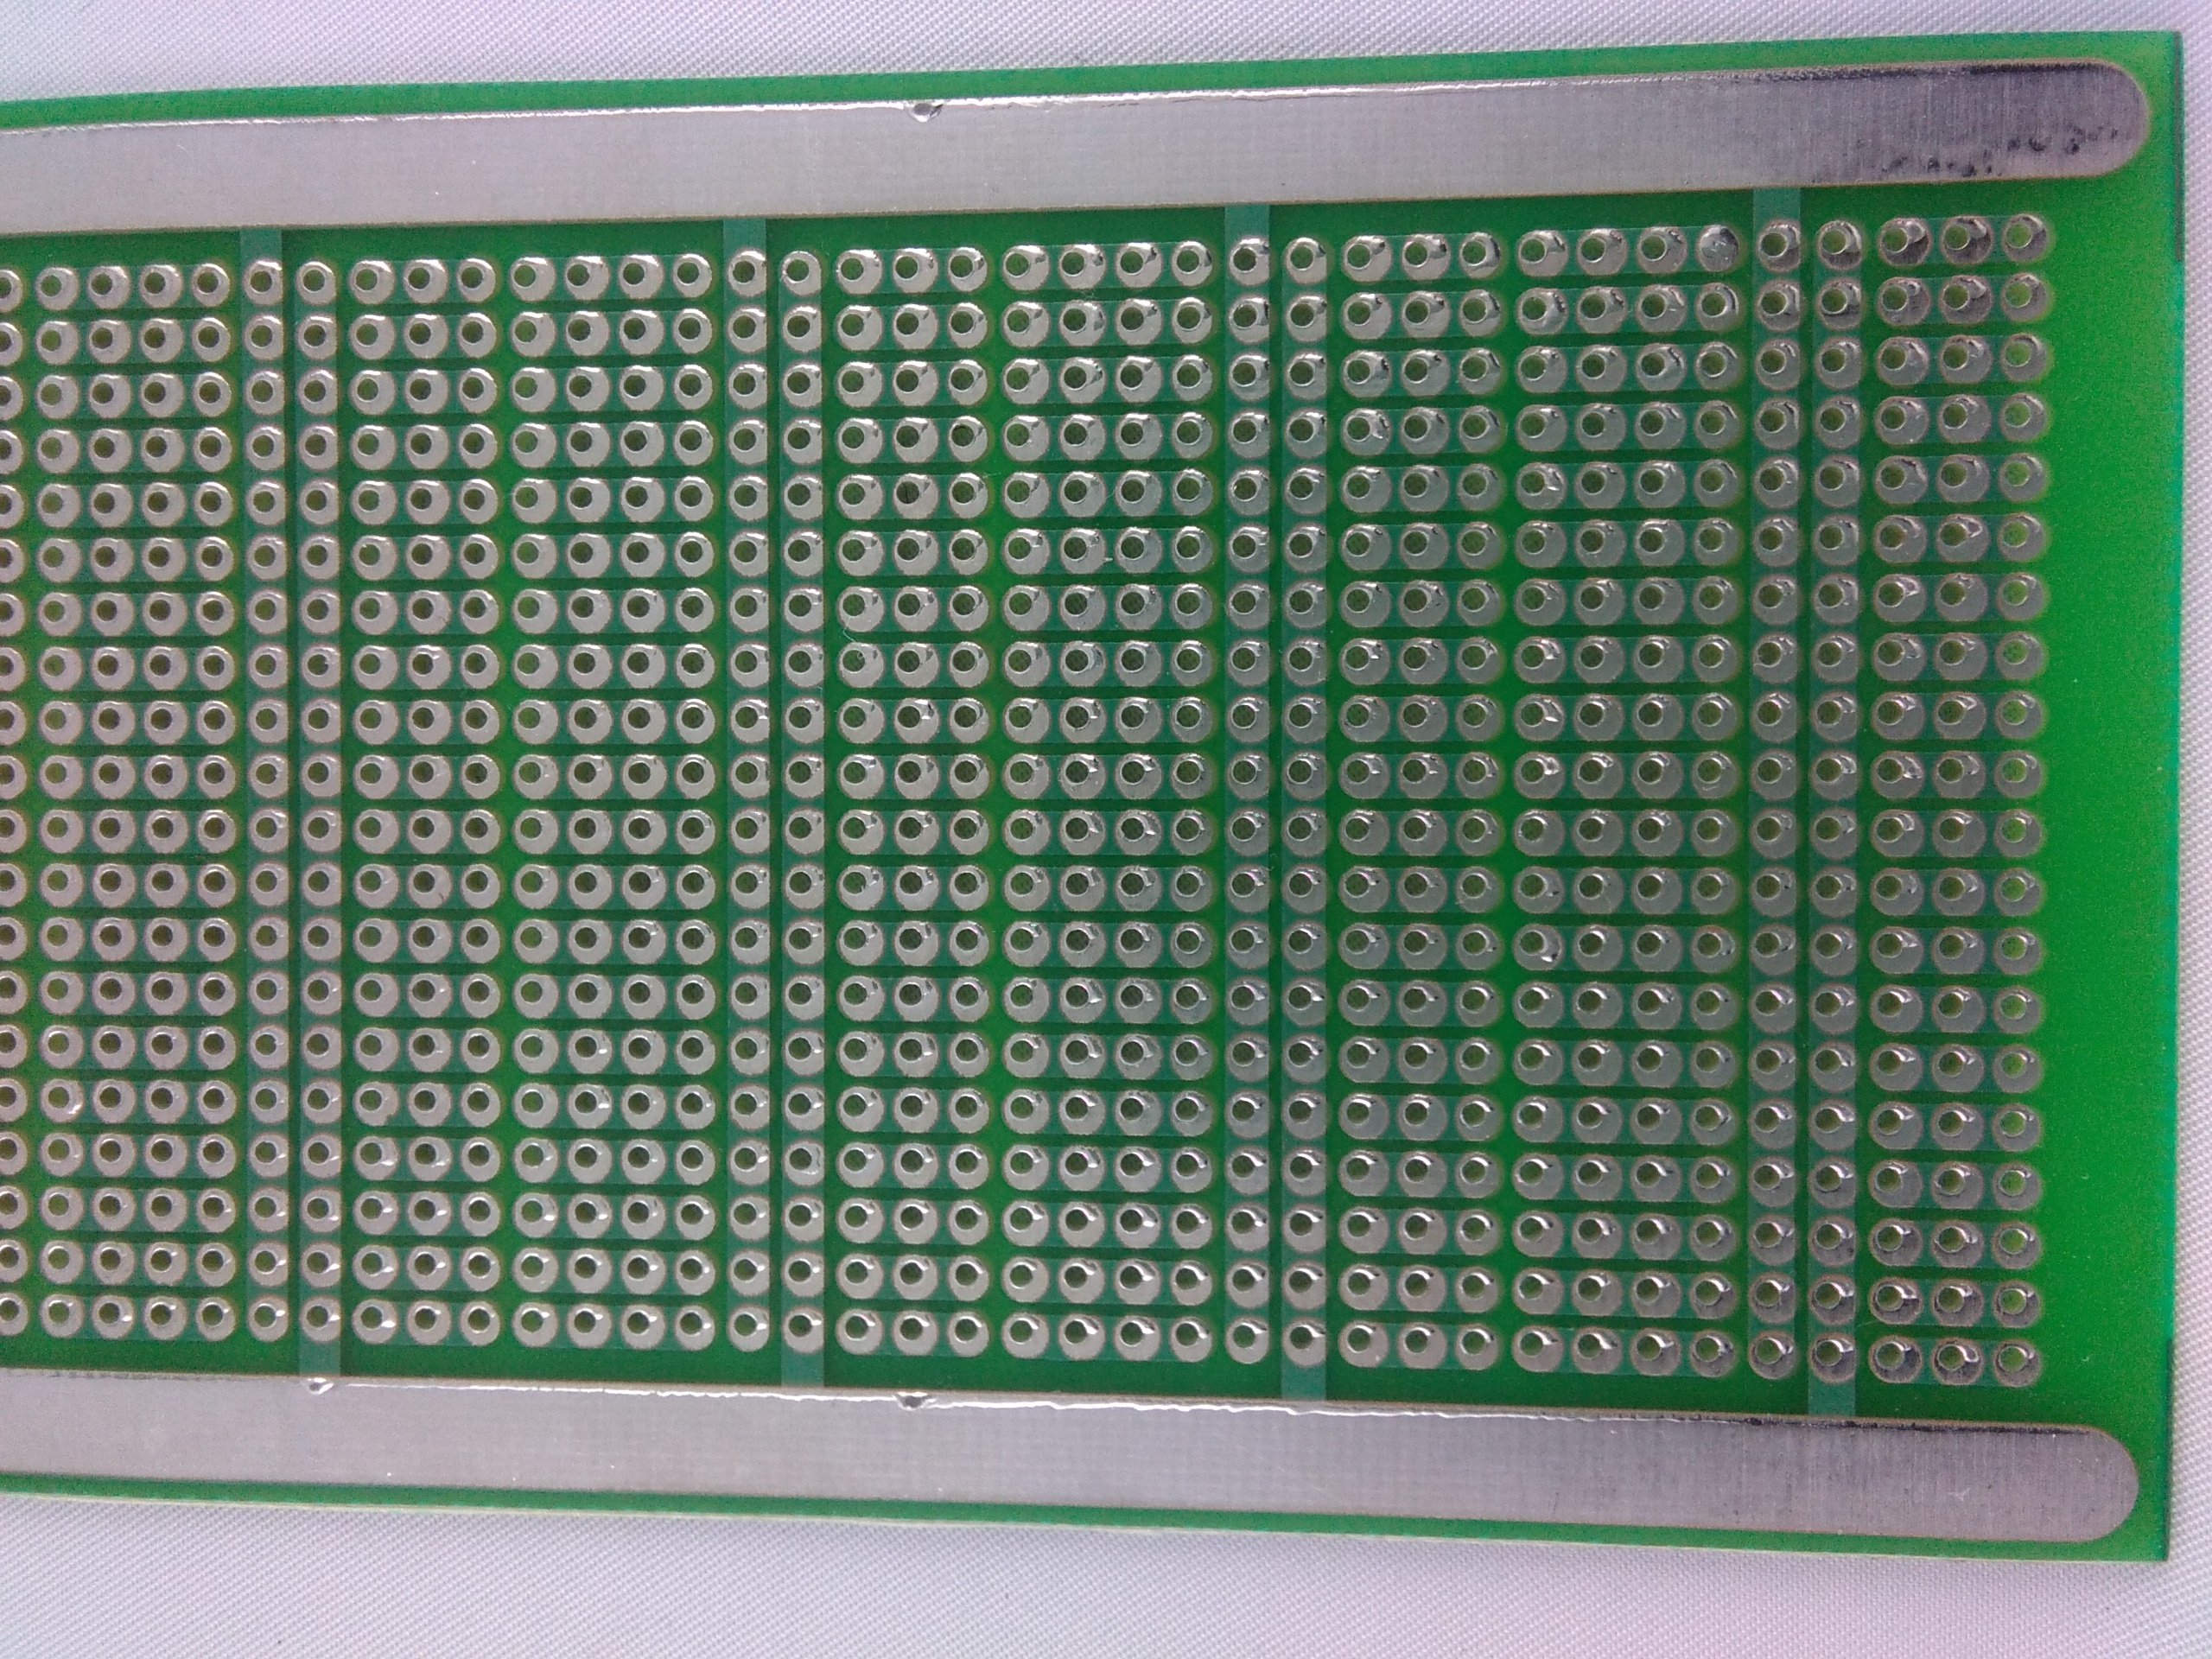
\includegraphics[scale=0.1,left]{universe.jpg}
  \caption{test figuwds}
  \label{fig:test}
\end{figure}

	%opis sygnalizatora świetlnego
	%\section{zestaw do kupienia}
		\subsection {Od czego zacząć}
			Wielu z nas nie ma nawet miernika w domu, myślę że to jest dobry moment na zakupienie takiego urządzenia. Będziemy wyglądać bardziej profesjonalnie. Poza tak oczywistym zakupem musimy mieć jeszcze kilka rzeczy o których dowiecie się w kolejnych częściach.
	\subsection{budowa}
	Przy pomocy Arduino jesteśmy w stanie tworzyć bardzo skomplikowane rzeczy ale ono nie jest do tego przystosowane. Głównym zastosowaniem jest tj inteligenty dom.
	\subsection{budowa}

\section {Zastosowanie elektroniki w życiu codziennym }
	 %sygnalizacja  świetlna drukarki, zmywarki,samochody, sprzęt gospodarstwa domowego, telefony,

\section {Więcej}

\subsection {Jak wiedzieć więcej}
Internet jest pełen informacji ale nie zawsze jest je znaleźć. W tym celu powstały różne fora, poradniki i blogi, które pomagają nam. Polecam szukać w języku angielski (nasze problemy wpisywać po w Google po angielsku np. How to include new library to Arduino). Gdy to zrobimy najlepiej szukać odpowiedzi na forum Stackoverflow. Serwis ma ponad 10 milionów artykułów, dzięki czemu jest duża szansa, że ktoś kiedyś miał taki sam problem jak wy. Stackoverflow można nazwać Wikipedią dla informatyków. 
\subsection{System kontroli wersji}
System kontroli wersji to oprogramowanie, które pomaga śledzić zmiany w kodzie źródłowym.
Dzięki temu mamy dostęp do kodu który kiedyś napisaliśmy (i został zmieniony/usunięty). Możemy również całkowicie zmieniać kod bez obawy, że przestanie on działać (w każdym momencie możemy przywrócić poprzednią wersję). Jest stosowany w dużych korporacjach, ponieważ ułatwia wspólną pracę. Jest kilka systemów kontroli wersji na rynku ale najbardziej popularnym (i polecanym przez nas) jest GitHub. Jako przykład możemy dodać, że został on wykorzystany do pisania tej pracy. W załącznikach na końcu będzie link do serwisu i do naszych repozytoriów (nie ważne, że nie macie pojęcia co to oznacza. Musicie po prostu wejść).
\cite{SKW-Wiki, Git-Wiki}
\subsection{}
%jak szukać bibliotek do czujników
%system kontroli wersji
%%
%\begin{thebibliography}{3}
%\bibitem{diller} Antoni Diller, \textit{\LaTeX\ wiersz po wierszu},
%wydawnictwo Helion, Gliwice 2001
%\bibitem{grfguide} D.P. Carlisle, \textit{Packages in the ‘graphics’
%bundle}
%\bibitem{lshort} Tobias Oetiker, \textit{The Not So Short Introduction
%To \LaTeX2e}
%\end{thebibliography}

%\nocite{*}


\newpage
\bibliography{abib} 
\bibliographystyle{ieeetr}

\end{document}

